\FloatBarrier
\subsection{Appendix A: Seismic measurement results}
All the seismic measurements have been made possible with the dedication and help from a vast number of locals. To all the people that have provided their expertise, time and assistance we would like to extend a sincere thank you. Due to the extent of the research it is impractical to list all those people but we would like to thank a few people in particular. For fruitful discussions and advice as well as facilitating measurements at the Heimansgroeve we thank Reinoud Sleeman and his colleagues from the KNMI. We also acknowledge their help in obtaining data from the Virtual European Broadband Seismograph Network (VEBSN). The measurements in Hungary were generously supported by Istvan Racz of the RMKI, Budapest, and the mining company MECSEK-\"OKO. For assistance during the measurements in Romania we are grateful to Romul Mircea Margineanu and the Salrom mining company. The Frejus tunnel measurements were kindly facilitated by Michel Zampaolo of the Laboratoire Souterrain de Modane. We thank Alessandro Bettini and Jose Jimenez of the Canfranc Underground Laboratory for their help during measurements in Spain. We are grateful to Fulvio Ricci, his colleagues from University ``Sapienza'' and the miners of IGEA spa, for access to the Sardinian site. We would also like to thank Eugenio Coccia and Benedetto Gallese for their help during measurements at the Gran Sasso underground laboratory. We are very grateful to Rudolf Widmer-Schnidrig, Thomas Forbinger and Walter Zuern of the Black Forest Observatory for the interesting discussions and access to their laboratory. We acknowledge Guido Nuijton for his thoughts on sites in Finland. For measurements carried out at the CLIO site in Japan we thank, Kazuaki Kuroda, Uchiyama Takashi, Osamu Miyakawa and Miyoki Shinji. Ricardo de Salvo and friends at the Italkali mine in Sicilie kindly assisted the measurements there. Finally we would like to acknowledge the help of EURIDICE staff members, Philippe van Marcke and Kris Moerkens, during measurements in Belgium.

\pagebreak
\FloatBarrier
\subsubsection*{Germany - Black forest}
\begin{figure}[h]
\centering
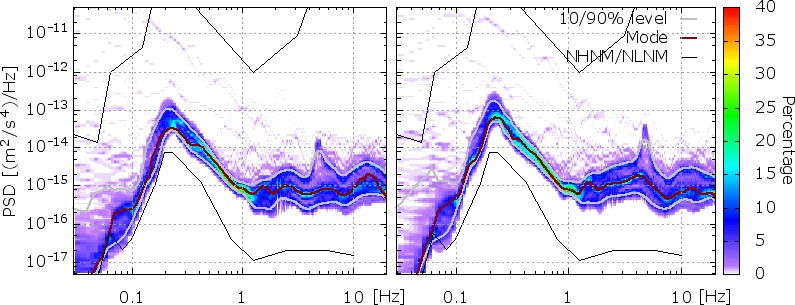
\includegraphics[width=\textwidth]{./Sec_SiteInfra/Figures/results/ZWald-A_multiplot1}
\caption{The horizontal component (left) and the vertical component (right) power spectral density plotted as a spectral variation from the Germany - Black forest site.}
\label{fig:ZWald-A_multiplot1}
\end{figure}\begin{figure}[h]
\centering
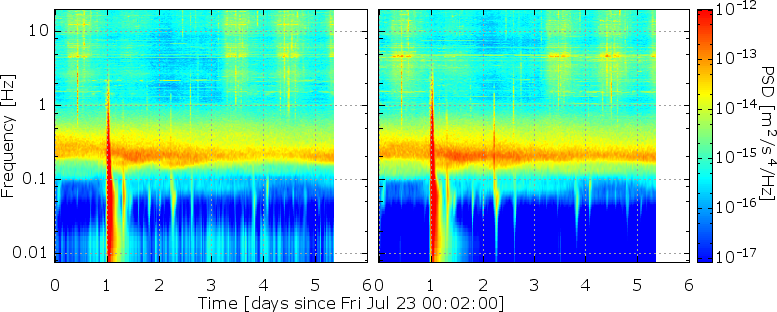
\includegraphics[width=\textwidth]{./Sec_SiteInfra/Figures/results/ZWald-A_multiplot2}
\caption{The spectrogram of the horizontal (left) and vertical (right) component from the Germany - Black forest site.}
\label{fig:ZWald-A_multiplot2}
\end{figure}

\pagebreak
\FloatBarrier
\subsubsection*{Spain - Laboratorio Subterr\'eneo de Canfranc}
\begin{figure}[h]
\centering
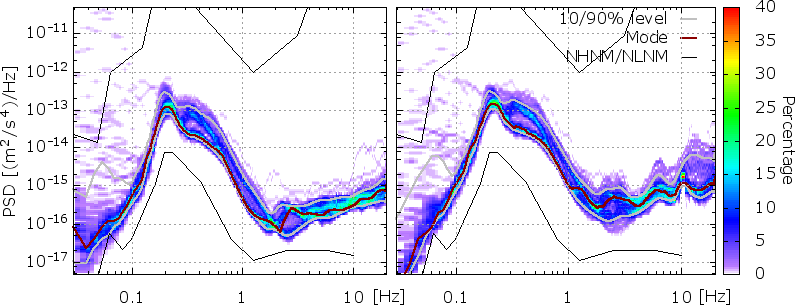
\includegraphics[width=\textwidth]{./Sec_SiteInfra/Figures/results/Canfranc-B_multiplot1}
\caption{The horizontal component (left) and the vertical component (right) power spectral density plotted as a spectral variation from the Spain - Laboratorio Subterr\'eneo de Canfranc site.}
\label{fig:Canfranc-B_multiplot1}
\end{figure}\begin{figure}[h]
\centering
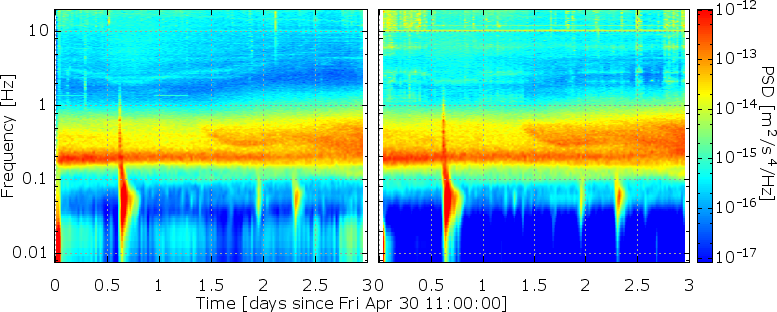
\includegraphics[width=\textwidth]{./Sec_SiteInfra/Figures/results/Canfranc-B_multiplot2}
\caption{The spectrogram of the horizontal (left) and vertical (right) component from the Spain - Laboratorio Subterráneo de Canfranc site.}
\label{fig:Canfranc-B_multiplot2}
\end{figure}

\pagebreak
\FloatBarrier
\subsubsection*{Finland - Sumiainen}
\begin{figure}[h]
\centering
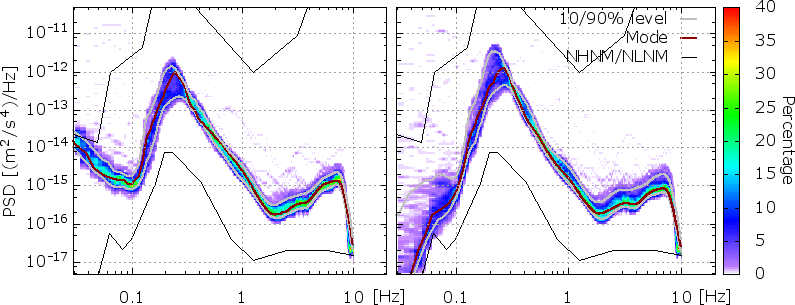
\includegraphics[width=\textwidth]{./Sec_SiteInfra/Figures/results/SUF_multiplot1}
\caption{The horizontal component (left) and the vertical component (right) power spectral density plotted as a spectral variation from the Finland - Sumiainen site.}
\label{fig:_multiplot1c}
\end{figure}\begin{figure}[h]
\centering
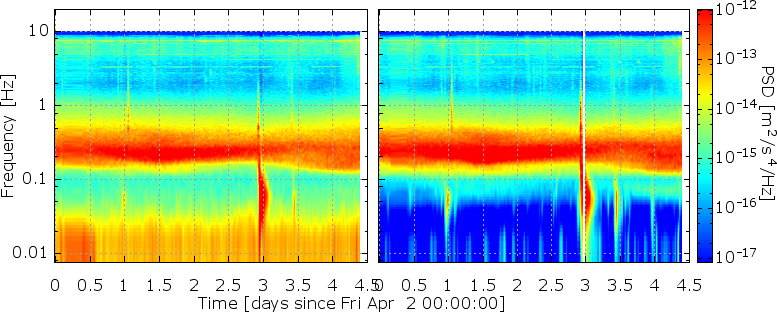
\includegraphics[width=\textwidth]{./Sec_SiteInfra/Figures/results/SUF_multiplot2}
\caption{The spectrogram of the horizontal (left) and vertical (right) component from the Finland - Sumiainen site.}
\label{fig:_multiplot2c}
\end{figure}

\pagebreak
\FloatBarrier
\subsubsection*{France - Frejus}
\begin{figure}[h]
\centering
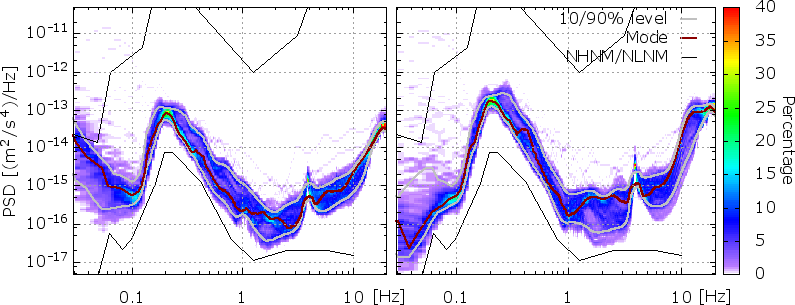
\includegraphics[width=\textwidth]{./Sec_SiteInfra/Figures/results/Frejus-A_multiplot1}
\caption{The horizontal component (left) and the vertical component (right) power spectral density plotted as a spectral variation from the France - Frejus site.}
\label{fig:Frejus-A_multiplot1}
\end{figure}\begin{figure}[h]
\centering
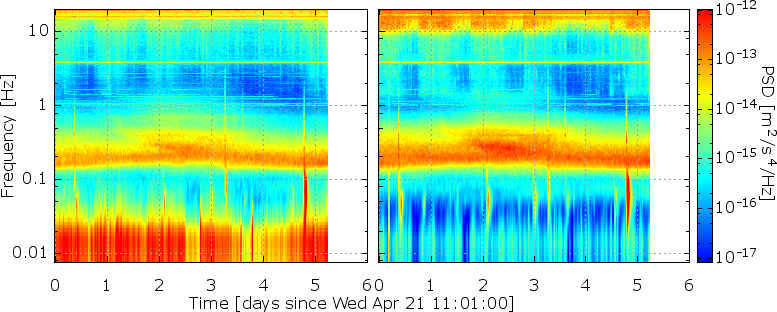
\includegraphics[width=\textwidth]{./Sec_SiteInfra/Figures/results/Frejus-A_multiplot2}
\caption{The spectrogram of the horizontal (left) and vertical (right) component from the France - Frejus site.}
\label{fig:Frejus-A_multiplot2}
\end{figure}

\pagebreak
\FloatBarrier
\subsubsection*{Italy - Gran Sasso}
\begin{figure}[h]
\centering
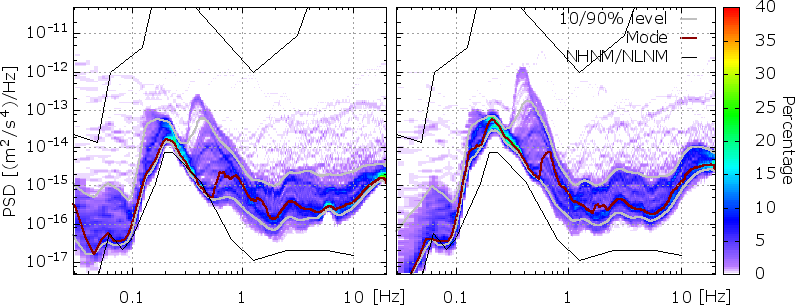
\includegraphics[width=\textwidth]{./Sec_SiteInfra/Figures/results/GSasso-A_multiplot1}
\caption{The horizontal component (left) and the vertical component (right) power spectral density plotted as a spectral variation from the Italy - Gran Sasso site.}
\label{fig:GSasso-A_multiplot1}
\end{figure}\begin{figure}[h]
\centering
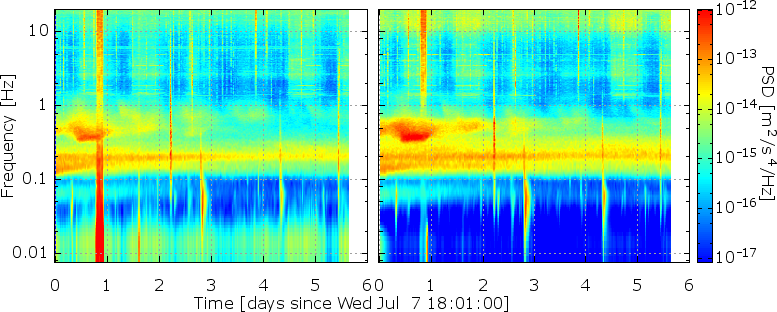
\includegraphics[width=\textwidth]{./Sec_SiteInfra/Figures/results/GSasso-A_multiplot2}
\caption{The spectrogram of the horizontal (left) and vertical (right) component from the Italy - Gran Sasso site.}
\label{fig:GSasso-A_multiplot2}
\end{figure}

\pagebreak
\FloatBarrier
\subsubsection*{Japan - Kamioka mine}
\begin{figure}[h]
\centering
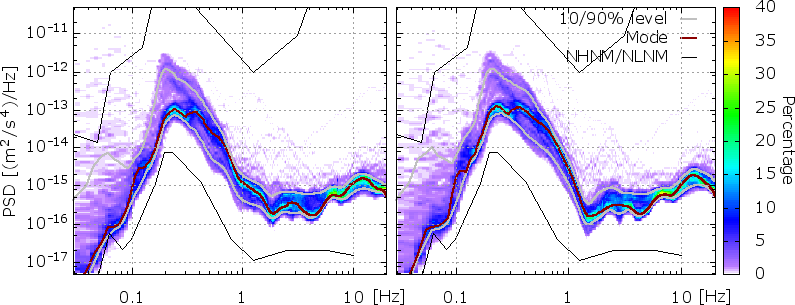
\includegraphics[width=\textwidth]{./Sec_SiteInfra/Figures/results/Kamioka-A_multiplot1}
\caption{The horizontal component (left) and the vertical component (right) power spectral density plotted as a spectral variation from the Japan - Kamioka mine site.}
\label{fig:Kamioka-A_multiplot1}
\end{figure}\begin{figure}[h]
\centering
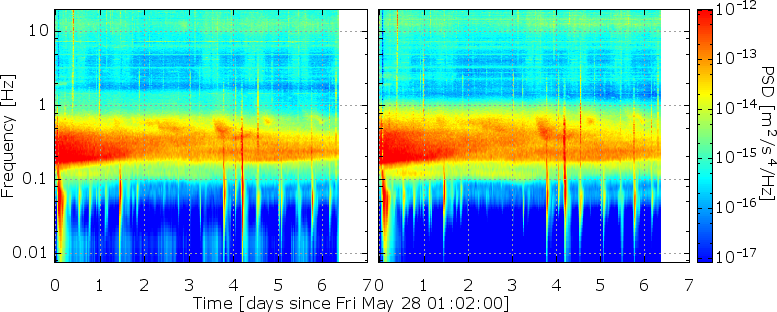
\includegraphics[width=\textwidth]{./Sec_SiteInfra/Figures/results/Kamioka-A_multiplot2}
\caption{The spectrogram of the horizontal (left) and vertical (right) component from the Japan - Kamioka mine site.}
\label{fig:Kamioka-A_multiplot2}
\end{figure}

\pagebreak
\FloatBarrier
\subsubsection*{Germany - Moxa}
\begin{figure}[h]
\centering
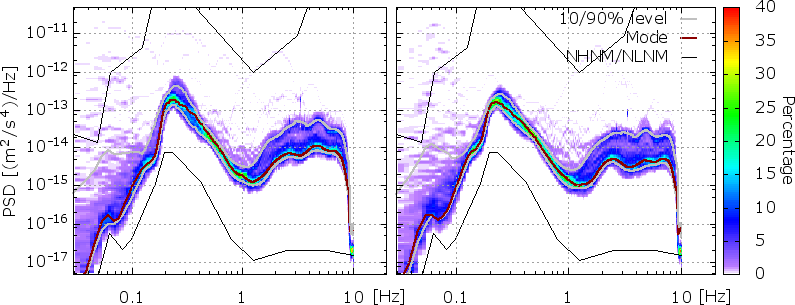
\includegraphics[width=\textwidth]{./Sec_SiteInfra/Figures/results/MOX_multiplot1}
\caption{The horizontal component (left) and the vertical component (right) power spectral density plotted as a spectral variation from the Germany - Moxa site.}
\label{fig:_multiplot1d}
\end{figure}\begin{figure}[h]
\centering
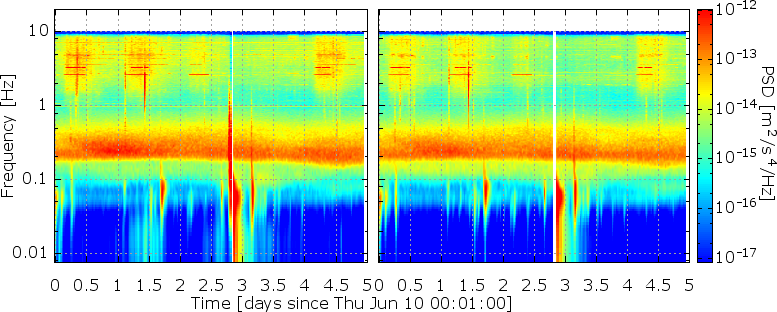
\includegraphics[width=\textwidth]{./Sec_SiteInfra/Figures/results/MOX_multiplot2}
\caption{The spectrogram of the horizontal (left) and vertical (right) component from the Germany - Moxa site.}
\label{fig:_multiplot2d}
\end{figure}

\pagebreak
\FloatBarrier
\subsubsection*{Netherlands - Heimansgroeve}
\begin{figure}[h]
\centering
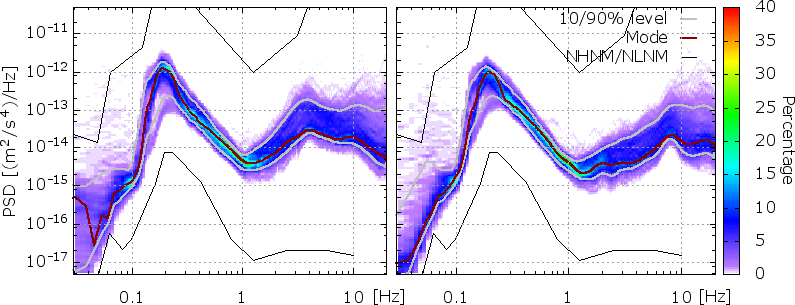
\includegraphics[width=\textwidth]{./Sec_SiteInfra/Figures/results/Heimans-A_multiplot1}
\caption{The horizontal component (left) and the vertical component (right) power spectral density plotted as a spectral variation from the Netherlands - Heimansgroeve site.}
\label{fig:Heimans-A_multiplot1}
\end{figure}\begin{figure}[h]
\centering
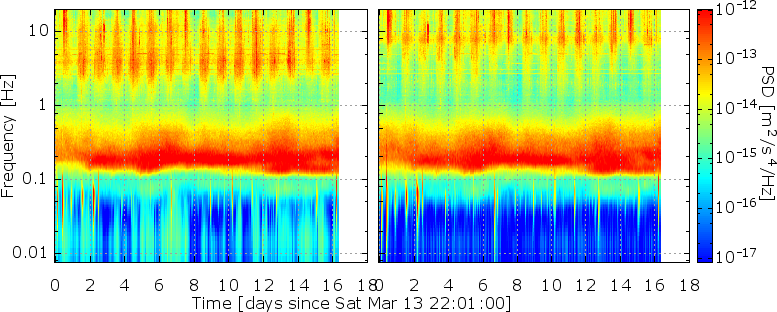
\includegraphics[width=\textwidth]{./Sec_SiteInfra/Figures/results/Heimans-A_multiplot2}
\caption{The spectrogram of the horizontal (left) and vertical (right) component from the Netherlands - Heimansgroeve site.}
\label{fig:Heimans-A_multiplot2}
\end{figure}

\pagebreak
\FloatBarrier
\subsubsection*{Romania - Slanic-Prahova}
\begin{figure}[h]
\centering
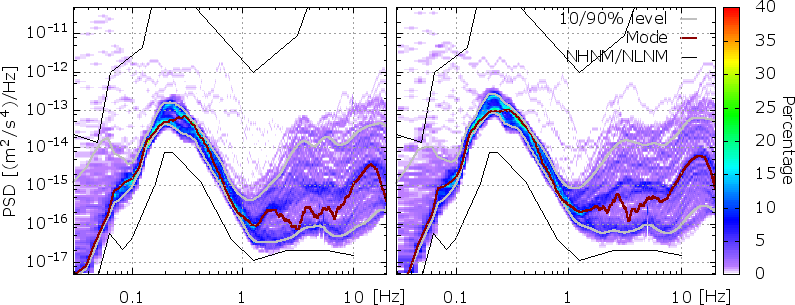
\includegraphics[width=\textwidth]{./Sec_SiteInfra/Figures/results/Slanic-A_multiplot1}
\caption{The horizontal component (left) and the vertical component (right) power spectral density plotted as a spectral variation from the Romania - Slanic-Prahova site.}
\label{fig:Slanic-A_multiplot1}
\end{figure}\begin{figure}[h]
\centering
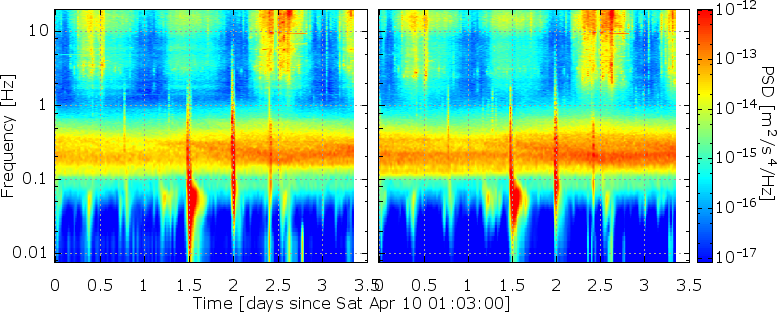
\includegraphics[width=\textwidth]{./Sec_SiteInfra/Figures/results/Slanic-A_multiplot2}
\caption{The spectrogram of the horizontal (left) and vertical (right) component from the Romania - Slanic-Prahova site.}
\label{fig:Slanic-A_multiplot2}
\end{figure}

\pagebreak
\FloatBarrier
\subsubsection*{Belgium - Mol}
\begin{figure}[h]
\centering
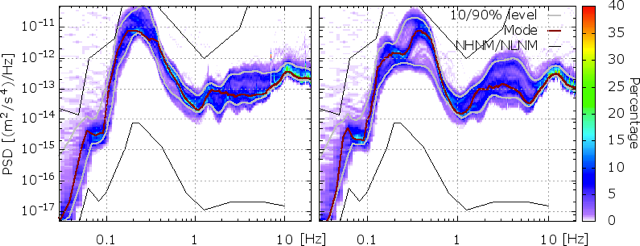
\includegraphics[width=\textwidth]{./Sec_SiteInfra/Figures/results/Mol-A_multiplot1}
\caption{The horizontal component (left) and the vertical component (right) power spectral density plotted as a spectral variation from the Romania - Slanic-Prahova site.}
\label{fig:Slanic-A_multiplot1}
\end{figure}\begin{figure}[h]
\centering
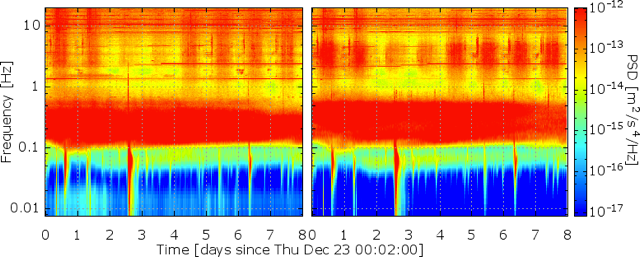
\includegraphics[width=\textwidth]{./Sec_SiteInfra/Figures/results/Mol-A_multiplot2}
\caption{The spectrogram of the horizontal (left) and vertical (right) component from the Romania - Slanic-Prahova site.}
\label{fig:Slanic-A_multiplot2}
\end{figure}
\FloatBarrier
\subsection{Appendix B: ET infrastructure drawings}


